\documentclass[a4paper]{article}
\usepackage[pdftex]{graphicx}
\usepackage[utf8]{inputenc}
\usepackage{enumerate}
\usepackage{siunitx}
\sisetup{locale=DE}
\usepackage{icomma}
\usepackage{amssymb}
\usepackage{tikz}
\usepackage{href-ul}
\hypersetup{
	colorlinks=true,
	linkcolor=blue,
	urlcolor=blue}
\usepackage{geometry}
\geometry{a4paper, top=15mm, left=15mm, right=15mm, bottom=15mm,
	headsep=10mm, footskip=12mm}

\begin{document}
	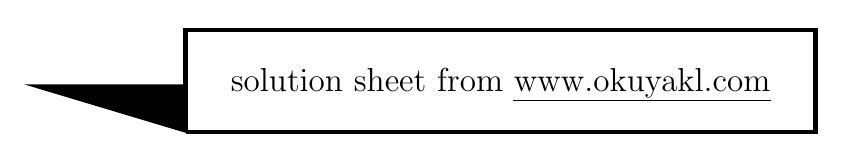
\begin{tikzpicture}(10,3)
		\draw[ultra thick](2,0) --(10,0) -- (10,1.3) --(2,1.3) -- (2,0);
		\draw[fill=black](2,0)-- (0,.6) -- (2,.6) -- (2,0);
		\node at (6,.6) {\large solution sheet from \href{http://www.okuyakl.com}{www.okuyakl.com}};
	\end{tikzpicture}
	\vspace{0.5 cm}
	
	\noindent{\bf Task 1.}\\
	\begin{minipage}{0.65\textwidth}
		The total resistance consists of the ohmic resistance of the capacitor $R$ on the real axis and the reactance of the capacitor $X=-{ 1 \over \omega C}$ on the imaginary axis. According to the Pythagorean theorem, the magnitude of the complex total resistance $Z$ is:
		$$
		\begin{array}{rcll}
			Z^2 & = & R^2 + \left( { 1 \over \omega C} \right)^2\\
			Z^2 & = & R^2 + \left( { 1 \over 2\pi f \cdot C} \right)^2\\
			Z & = & \sqrt{R^2 + \left( { 1 \over 4\pi^2 f^2 \cdot C^2} \right)}
		\end{array}
		$$
	\end{minipage}
	\begin{minipage}{0.35\textwidth}
		\includegraphics[width=6 cm]{zeidi234.pdf}
	\end{minipage}
	\vspace{0.5 cm}
	
	\noindent{\bf Task 2. a)}\\
	If the voltage $U_{R,1}$ drops across the ohmic resistor, a current of the strength flows through it:
	$$ I = {U \over R} = {\SI{11,2}{\volt} \over \SI{40e3}{\ohm}} = \SI{0.28}{\milli\ampere}$$
	According to the phasor diagram, the effective voltage that drops across the capacitor is:
	$$
	\begin{array}{rcll}
		U_{C,1}^2 & = & U_{eff}^2 - U_{R,1}^2 \\
		U_{C,1} & = & \sqrt{U_{eff}^2 - U_{R,1}^2 }\\
		U_{C,1} & = & \sqrt{(\SI{12}{\volt})^2 - (\SI{11,2}{\volt})^2} = \SI{4,3} {\volt}
	\end{array}
	$$
	This results in a reactance of
	$$X = {\SI{4.3}{\volt} \over \SI{0.28}{\milli\ampere}}= \SI{15.4}{\kilo\ohm} $$
	We equate $X={ 1 \over \omega C}$ and solve for $C$:
	$$C = {1 \over 2\pi f X} = {{1 \over 2\pi \cdot \SI{520}{\hertz} \cdot \SI{15,4e3}{\ohm}}} = \SI{20e-9}{\farad} = \SI{20}{\nano\farad}$$
	Unit check:
	$$\SI{}{1 \over {\second^{-1}\cdot \volt \cdot \ampere^{-1}}}= \SI{}{\ampere\second \over \volt} = F $$
	The following applies to the phase shift $\varphi_1$ between current and input voltage:
	$$\tan\varphi_1= {X \over R} \quad \Rightarrow \quad \varphi_1 = \arctan\left({X \over R} \right)= \arctan \left({\SI{15,4} {\kilo\ohm} \over \SI{40}{\kilo\ohm}} \right) = 21^\circ$$
	\vspace{0.5 cm}
	
	\noindent{\bf Task 2. b)}\\
	The active power $P_1$ is the power that is converted into Joule heat at the ohmic resistance:
	$$P_1 = {U_{R,eff,1}^2 \over R} = {(\SI{11,2}{\volt})^2 \over \SI{40e3}{\ohm}} = \SI{3,1}{\milli\watt}$$
	\vspace{0.5 cm}
	
	\noindent{\bf Task 3. a)}\\
	Since it is a series connection, the current $I_eff$ is the same in the entire circuit according to Kirchhoff's law; So the frequency-dependent effective current $I_{R,eff}(f)$ is equal to the effective total current $I_{eff}$:
	$$
	\renewcommand{\arraystretch}{2}
	\begin{array}{rcll}
		I_{R,eff}(f) & = & I_{eff} \\
		{U_{R,eff}(f) \over R} & = & {U_{eff}\over Z} &|\cdot R\\
		U_{R,eff}(f) & = & {R \over Z} \cdot U_{eff} \\
		U_{R,eff}(f) & = & {R \over \sqrt{R^2 + {1 \over 4 \pi^2 C^2} \cdot {1 \over f^2}}} \cdot U_{eff}
	\end{array}
	$$
	\vspace{0.5 cm}
	
	\noindent{\bf Task 3. b)}\\
	If the effective values of the voltages on the capacitor and on the ohmic resistor are the same, we conclude for the cutoff frequency:
	$$
	\renewcommand{\arraystretch}{2}
	\begin{array}{rcll}
		\varphi & = & 45^\circ \Rightarrow & X = R \\
		R & = & {1 \over 2 \pi f \cdot C} & | \cdot f \quad :R\\
		f_g & = & {1 \over 2 \pi R \cdot C}\\
		f_g & = & {1 \over 2 \pi \cdot \SI{40e3}{\ohm} \cdot \SI{20e-9}{\farad}}\\
		f_g & = & \SI{200}{\hertz}
	\end{array}
	$$
	Unit check:
	$$\SI{}{1 \over \volt\cdot \ampere^{-1}\cdot \ampere\cdot \second \cdot \volt^{-1}}= \SI{}{\second^{- 1}}=\SI{}{\hertz}$$
	The effective values of the voltages $U_{R,eff}$ and $U_{C_eff}$ are the same; Added vectorially they result in $U_{eff}=\SI{12}{\volt}$. So is:
	$$
	\renewcommand{\arraystretch}{2}
	\begin{array}{rcll}
		U_{eff}^2 & = & U_{R,eff}^2+ U_{C_eff}^2 & | U_{R,eff} = U_{C_eff}\\
		U_{eff}^2 & = & 2\cdot U_{R,eff}^2 &| \sqrt{\quad} \\
		U_{eff} & = & \sqrt{2} \cdot U_{R,eff} \\
		U_{R,eff} & = & {U_{eff} \over \sqrt{2}} \\
		U_{R,eff} & = & {\SI{12}{\volt} \over \sqrt{2}} & = \SI{8.5}{\volt} = U_{C_eff}
	\end{array}
	$$
	Both effective values have the value $\SI{8.5}{\volt}$.
	\vspace{0.5 cm}
	
	\noindent{\bf Task 3. c)}\\
	If the frequency $f$ becomes very large, then the second summand approaches
	zero under the root and thus the factor ${R \over Z}\approx 1$ before $U_{eff}$. This becomes the two voltage values left and right practically the same size. This also coincides with the fact that the capacitor conducts better and better as the frequency increases, until finally at very high frequencies its resistance becomes negligibly small compared to the preceding ohmic resistance.
	
	\begin{center}
		\includegraphics[width=7 cm]{../../viecher/eendcomic.pdf}
		
		Here you can go back to the \href{https://www.okuyakl.de/phys/p13wekoL234/ae234.pdf}{task sheet}
	\end{center}
	
	\end{document}